% ---
\subsection{Figuras}
\label{sec_figuras}
% ---

\index{figuras}Figuras podem ser criadas diretamente em \LaTeX,
como o exemplo da \autoref{fig_circulo}, ou inseridas a partir de arquivos externos como a \autoref{fig_logo}, que é o Logotipo do \ac{ifsp}. \index{logotipo}

As figuras externas devem possuir boa qualidade e preferencialmente serem vetorizadas para se obter o melhor resultado. Procure criar suas imagens e diagramas pensando em utilizar impressão em preto-e-branco ou escala de cinza. Isto é importante, principalmente quando se pretende publicar o trabalho, uma vez que a maioria das publicações são somente em preto-e-branco. Outro benefício é o custo de impressão, normalmente menor para páginas preto-e-branco em relação a páginas coloridas.

Para diagramas em UML o PlantUML pode ser utilizado para gerar código \LaTeX como exemplo na  \autoref{diagramauml}.


Quando existem diversos detalhes utilize \ac{png} em vez de JPG \footnote{Abreviado de \ac{jpeg}}, observe a diferença no exemplo em \url{https://tex.stackexchange.com/questions/136087/selecting-best-file-extension-for-graphics-figures-pictures}.

O número da seção que contém as informações sobre figuras é \ref{sec_figuras}.


\begin{figure}[htb]
	\begin{center}
	    \setlength{\unitlength}{5cm}
		\begin{picture}(1,1)
		\put(0,0){\line(0,1){1}}
		\put(0,0){\line(1,0){1}}
		\put(0,0){\line(1,1){1}}
		\put(0,0){\line(1,2){.5}}
		\put(0,0){\line(1,3){.3333}}
		\put(0,0){\line(1,4){.25}}
		\put(0,0){\line(1,5){.2}}
		\put(0,0){\line(1,6){.1667}}
		\put(0,0){\line(2,1){1}}
		\put(0,0){\line(2,3){.6667}}
		\put(0,0){\line(2,5){.4}}
		\put(0,0){\line(3,1){1}}
		\put(0,0){\line(3,2){1}}
		\put(0,0){\line(3,4){.75}}
		\put(0,0){\line(3,5){.6}}
		\put(0,0){\line(4,1){1}}
		\put(0,0){\line(4,3){1}}
		\put(0,0){\line(4,5){.8}}
		\put(0,0){\line(5,1){1}}
		\put(0,0){\line(5,2){1}}
		\put(0,0){\line(5,3){1}}
		\put(0,0){\line(5,4){1}}
		\put(0,0){\line(5,6){.8333}}
		\put(0,0){\line(6,1){1}}
		\put(0,0){\line(6,5){1}}
		\end{picture}
	\end{center}
	\caption{\label{fig_circulo}A delimitação do espaço}
	\fonte{Os Autores}
\end{figure}


\begin{figure}[htb]
    \centering
	
\includegraphics{\ifspprefixo/logo-02.jpg}
	\caption{\label{fig_logo}Logotipo \ac{ifsp}}
	\fonte{\ac{ifsp}}
\end{figure}



% generated by Plantuml 7997beta
\definecolor{plantucolor0000}{RGB}{254,254,206}
\definecolor{plantucolor0001}{RGB}{168,0,54}
\definecolor{plantucolor0002}{RGB}{173,209,178}
\definecolor{plantucolor0003}{RGB}{0,0,0}
\definecolor{plantucolor0004}{RGB}{0,0,255}

\begin{figure}[htb]
    \centering
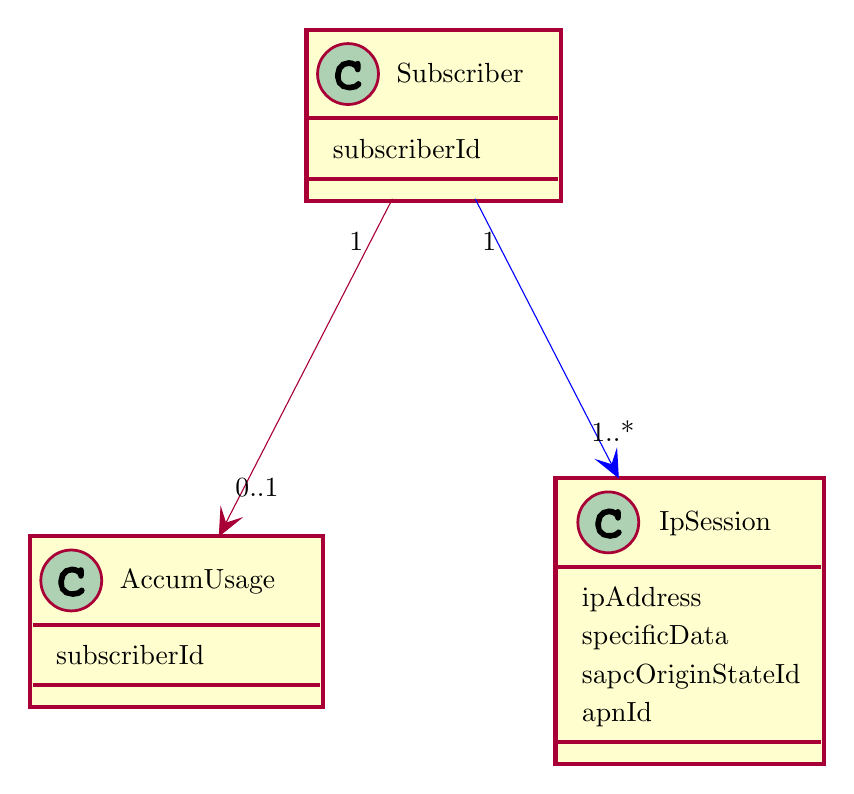
\begin{tikzpicture}[yscale=-1]
\draw[color=plantucolor0001,fill=plantucolor0000,line width=1.5pt] (131pt,29pt) rectangle (223pt,90.8359pt);
\draw[color=plantucolor0001,fill=plantucolor0002,line width=1.0pt] (146pt,45pt) ellipse (11pt and 11pt);
\draw[color=black,fill=black] (148.7656pt,40.875pt) ..controls (148.9219pt,40.6563pt) .. (149.1094pt,40.5469pt) ..controls (149.2969pt,40.4375pt) .. (149.5156pt,40.4375pt) ..controls (149.8906pt,40.4375pt) .. (150.125pt,40.6953pt) ..controls (150.3594pt,40.9531pt) .. (150.3594pt,41.5625pt) -- (150.3594pt,43.0156pt) ..controls (150.3594pt,43.625pt) .. (150.125pt,43.8906pt) ..controls (149.8906pt,44.1563pt) .. (149.5156pt,44.1563pt) ..controls (149.1719pt,44.1563pt) .. (148.9688pt,43.9531pt) ..controls (148.7656pt,43.7656pt) .. (148.6563pt,43.25pt) ..controls (148.6094pt,42.8906pt) .. (148.4219pt,42.7031pt) ..controls (148.0938pt,42.3281pt) .. (147.4844pt,42.1094pt) ..controls (146.875pt,41.8906pt) .. (146.25pt,41.8906pt) ..controls (145.4844pt,41.8906pt) .. (144.8516pt,42.2188pt) ..controls (144.2188pt,42.5469pt) .. (143.7266pt,43.2969pt) ..controls (143.2344pt,44.0469pt) .. (143.2344pt,45.0781pt) -- (143.2344pt,46.1719pt) ..controls (143.2344pt,47.4063pt) .. (144.125pt,48.2266pt) ..controls (145.0156pt,49.0469pt) .. (146.6094pt,49.0469pt) ..controls (147.5469pt,49.0469pt) .. (148.2031pt,48.7969pt) ..controls (148.5938pt,48.6406pt) .. (149.0156pt,48.2031pt) ..controls (149.2813pt,47.9375pt) .. (149.4297pt,47.8594pt) ..controls (149.5781pt,47.7813pt) .. (149.7813pt,47.7813pt) ..controls (150.1094pt,47.7813pt) .. (150.3672pt,48.0391pt) ..controls (150.625pt,48.2969pt) .. (150.625pt,48.6406pt) ..controls (150.625pt,48.9844pt) .. (150.2813pt,49.3906pt) ..controls (149.7813pt,49.9688pt) .. (148.9844pt,50.2969pt) ..controls (147.9063pt,50.75pt) .. (146.6094pt,50.75pt) ..controls (145.0938pt,50.75pt) .. (143.8906pt,50.125pt) ..controls (142.9063pt,49.625pt) .. (142.2188pt,48.5547pt) ..controls (141.5313pt,47.4844pt) .. (141.5313pt,46.2031pt) -- (141.5313pt,45.0469pt) ..controls (141.5313pt,43.7188pt) .. (142.1484pt,42.5703pt) ..controls (142.7656pt,41.4219pt) .. (143.8594pt,40.8047pt) ..controls (144.9531pt,40.1875pt) .. (146.1875pt,40.1875pt) ..controls (146.9219pt,40.1875pt) .. (147.5703pt,40.3516pt) ..controls (148.2188pt,40.5156pt) .. (148.7656pt,40.875pt);
\node at (160pt,37.4531pt)[below right]{Subscriber};
\draw[color=plantucolor0001,line width=1.5pt] (132pt,61pt) -- (222pt,61pt);
\node at (137pt,65pt)[below right]{subscriberId};
\draw[color=plantucolor0001,line width=1.5pt] (132pt,82.8359pt) -- (222pt,82.8359pt);
\draw[color=plantucolor0001,fill=plantucolor0000,line width=1.5pt] (31pt,212pt) rectangle (137pt,273.8359pt);
\draw[color=plantucolor0001,fill=plantucolor0002,line width=1.0pt] (46pt,228pt) ellipse (11pt and 11pt);
\draw[color=black,fill=black] (48.7656pt,223.875pt) ..controls (48.9219pt,223.6563pt) .. (49.1094pt,223.5469pt) ..controls (49.2969pt,223.4375pt) .. (49.5156pt,223.4375pt) ..controls (49.8906pt,223.4375pt) .. (50.125pt,223.6953pt) ..controls (50.3594pt,223.9531pt) .. (50.3594pt,224.5625pt) -- (50.3594pt,226.0156pt) ..controls (50.3594pt,226.625pt) .. (50.125pt,226.8906pt) ..controls (49.8906pt,227.1563pt) .. (49.5156pt,227.1563pt) ..controls (49.1719pt,227.1563pt) .. (48.9688pt,226.9531pt) ..controls (48.7656pt,226.7656pt) .. (48.6563pt,226.25pt) ..controls (48.6094pt,225.8906pt) .. (48.4219pt,225.7031pt) ..controls (48.0938pt,225.3281pt) .. (47.4844pt,225.1094pt) ..controls (46.875pt,224.8906pt) .. (46.25pt,224.8906pt) ..controls (45.4844pt,224.8906pt) .. (44.8516pt,225.2188pt) ..controls (44.2188pt,225.5469pt) .. (43.7266pt,226.2969pt) ..controls (43.2344pt,227.0469pt) .. (43.2344pt,228.0781pt) -- (43.2344pt,229.1719pt) ..controls (43.2344pt,230.4063pt) .. (44.125pt,231.2266pt) ..controls (45.0156pt,232.0469pt) .. (46.6094pt,232.0469pt) ..controls (47.5469pt,232.0469pt) .. (48.2031pt,231.7969pt) ..controls (48.5938pt,231.6406pt) .. (49.0156pt,231.2031pt) ..controls (49.2813pt,230.9375pt) .. (49.4297pt,230.8594pt) ..controls (49.5781pt,230.7813pt) .. (49.7813pt,230.7813pt) ..controls (50.1094pt,230.7813pt) .. (50.3672pt,231.0391pt) ..controls (50.625pt,231.2969pt) .. (50.625pt,231.6406pt) ..controls (50.625pt,231.9844pt) .. (50.2813pt,232.3906pt) ..controls (49.7813pt,232.9688pt) .. (48.9844pt,233.2969pt) ..controls (47.9063pt,233.75pt) .. (46.6094pt,233.75pt) ..controls (45.0938pt,233.75pt) .. (43.8906pt,233.125pt) ..controls (42.9063pt,232.625pt) .. (42.2188pt,231.5547pt) ..controls (41.5313pt,230.4844pt) .. (41.5313pt,229.2031pt) -- (41.5313pt,228.0469pt) ..controls (41.5313pt,226.7188pt) .. (42.1484pt,225.5703pt) ..controls (42.7656pt,224.4219pt) .. (43.8594pt,223.8047pt) ..controls (44.9531pt,223.1875pt) .. (46.1875pt,223.1875pt) ..controls (46.9219pt,223.1875pt) .. (47.5703pt,223.3516pt) ..controls (48.2188pt,223.5156pt) .. (48.7656pt,223.875pt);
\node at (60pt,220.4531pt)[below right]{AccumUsage};
\draw[color=plantucolor0001,line width=1.5pt] (32pt,244pt) -- (136pt,244pt);
\node at (37pt,248pt)[below right]{subscriberId};
\draw[color=plantucolor0001,line width=1.5pt] (32pt,265.8359pt) -- (136pt,265.8359pt);
\draw[color=plantucolor0001,fill=plantucolor0000,line width=1.5pt] (221pt,191pt) rectangle (318pt,294.3438pt);
\draw[color=plantucolor0001,fill=plantucolor0002,line width=1.0pt] (240.05pt,207pt) ellipse (11pt and 11pt);
\draw[color=black,fill=black] (242.8156pt,202.875pt) ..controls (242.9719pt,202.6563pt) .. (243.1594pt,202.5469pt) ..controls (243.3469pt,202.4375pt) .. (243.5656pt,202.4375pt) ..controls (243.9406pt,202.4375pt) .. (244.175pt,202.6953pt) ..controls (244.4094pt,202.9531pt) .. (244.4094pt,203.5625pt) -- (244.4094pt,205.0156pt) ..controls (244.4094pt,205.625pt) .. (244.175pt,205.8906pt) ..controls (243.9406pt,206.1563pt) .. (243.5656pt,206.1563pt) ..controls (243.2219pt,206.1563pt) .. (243.0188pt,205.9531pt) ..controls (242.8156pt,205.7656pt) .. (242.7063pt,205.25pt) ..controls (242.6594pt,204.8906pt) .. (242.4719pt,204.7031pt) ..controls (242.1438pt,204.3281pt) .. (241.5344pt,204.1094pt) ..controls (240.925pt,203.8906pt) .. (240.3pt,203.8906pt) ..controls (239.5344pt,203.8906pt) .. (238.9016pt,204.2188pt) ..controls (238.2688pt,204.5469pt) .. (237.7766pt,205.2969pt) ..controls (237.2844pt,206.0469pt) .. (237.2844pt,207.0781pt) -- (237.2844pt,208.1719pt) ..controls (237.2844pt,209.4063pt) .. (238.175pt,210.2266pt) ..controls (239.0656pt,211.0469pt) .. (240.6594pt,211.0469pt) ..controls (241.5969pt,211.0469pt) .. (242.2531pt,210.7969pt) ..controls (242.6438pt,210.6406pt) .. (243.0656pt,210.2031pt) ..controls (243.3313pt,209.9375pt) .. (243.4797pt,209.8594pt) ..controls (243.6281pt,209.7813pt) .. (243.8313pt,209.7813pt) ..controls (244.1594pt,209.7813pt) .. (244.4172pt,210.0391pt) ..controls (244.675pt,210.2969pt) .. (244.675pt,210.6406pt) ..controls (244.675pt,210.9844pt) .. (244.3313pt,211.3906pt) ..controls (243.8313pt,211.9688pt) .. (243.0344pt,212.2969pt) ..controls (241.9563pt,212.75pt) .. (240.6594pt,212.75pt) ..controls (239.1438pt,212.75pt) .. (237.9406pt,212.125pt) ..controls (236.9563pt,211.625pt) .. (236.2688pt,210.5547pt) ..controls (235.5813pt,209.4844pt) .. (235.5813pt,208.2031pt) -- (235.5813pt,207.0469pt) ..controls (235.5813pt,205.7188pt) .. (236.1984pt,204.5703pt) ..controls (236.8156pt,203.4219pt) .. (237.9094pt,202.8047pt) ..controls (239.0031pt,202.1875pt) .. (240.2375pt,202.1875pt) ..controls (240.9719pt,202.1875pt) .. (241.6203pt,202.3516pt) ..controls (242.2688pt,202.5156pt) .. (242.8156pt,202.875pt);
\node at (254.95pt,199.4531pt)[below right]{IpSession};
\draw[color=plantucolor0001,line width=1.5pt] (222pt,223pt) -- (317pt,223pt);
\node at (227pt,227pt)[below right]{ipAddress};
\node at (227pt,240.8359pt)[below right]{specificData};
\node at (227pt,254.6719pt)[below right]{sapcOriginStateId};
\node at (227pt,268.5078pt)[below right]{apnId};
\draw[color=plantucolor0001,line width=1.5pt] (222pt,286.3438pt) -- (317pt,286.3438pt);
\draw[color=plantucolor0004] (191.942pt,90.081pt) ..controls (205.204pt,115.893pt) and (224.952pt,154.325pt) .. (241.265pt,186.076pt);
\draw[color=plantucolor0004,fill=plantucolor0004] (243.646pt,190.709pt) -- (243.0894pt,180.8759pt) -- (241.3604pt,186.262pt) -- (235.9742pt,184.5329pt) -- (243.646pt,190.709pt) -- cycle;
\node at (191.0584pt,98.9168pt)[below right]{1};
\node at (230.3817pt,166.6703pt)[below right]{1..*};
\draw[color=plantucolor0001] (162.058pt,90.081pt) ..controls (145.645pt,122.023pt) and (119.302pt,173.295pt) .. (101.824pt,207.31pt);
\draw[color=plantucolor0001,fill=plantucolor0001] (99.5252pt,211.784pt) -- (107.1969pt,205.6078pt) -- (101.8108pt,207.337pt) -- (100.0816pt,201.9509pt) -- (99.5252pt,211.784pt) -- cycle;
\node at (143.0082pt,98.7264pt)[below right]{1};
\node at (101.801pt,187.522pt)[below right]{0..1};
\end{tikzpicture}
\caption{\label{diagramauml}Exemplo de Diagrama UML gerado a partir do PlantUML}
	\legend{Fonte: Os Autores}
\end{figure}

A \autoref{fig_diag_virado} exemplifica como utilizar uma imagem qualquer em formato paisagem (página inteira). Obs: Utilizamos a imagem de forma a ilustrar o procedimento. Considere a legibilidade da figura quando for utilizar no trabalho final.

Para casos onde a figura referenciada está muito distante por algum motivo é possível fazer uma referencia indicando a página : \autorefwithpage{fig_diag_virado}

\begin{sidewaysfigure}[htb]
    \centering
	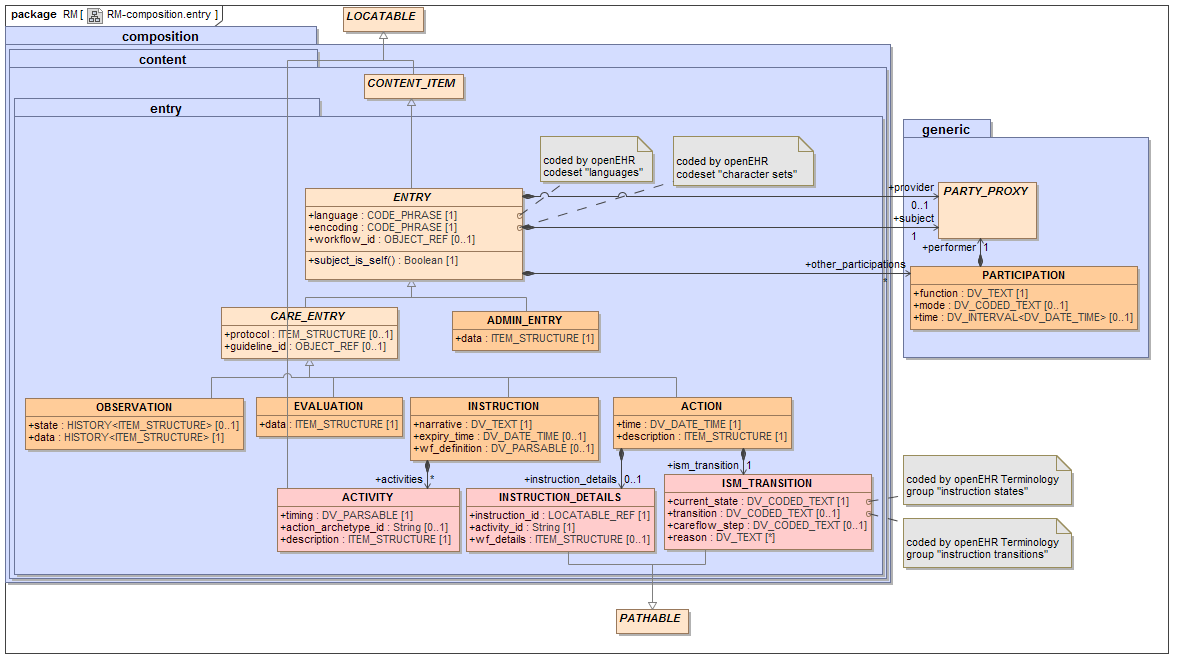
\includegraphics[width=0.9\textwidth]{exemplos/exemplo_diag_horizontal.png}
	\caption{\label{fig_diag_virado}Diagrama Virado - Exemplo}
	\fonte{\cite{openehrCompositionEntry}}
\end{sidewaysfigure}
